\section{lemma2(core)}

\begin{lemma}
\end{lemma}
Suppose we have a Riemann Sphere $C$ and two diagrams $(C,\iota,\xi)$,$(C',\iota',\xi')$, their regular cell complex refinements $\overline{(C,\iota,\xi)}$,$\overline{(C',\iota',\xi')}$ and sheaves $\mathfrak{F}$,$\mathfrak{F}'$ on them such that they differ only on a small disk $D\subset C$.\\

Below figures show only $\mathfrak{F}$,$\mathfrak{F}'$ restricted to $D$.
\begin{figure}[H] % Optional: [h] means here, [t] for top, [b] for bottom, [p] for page of floats
    \centering
    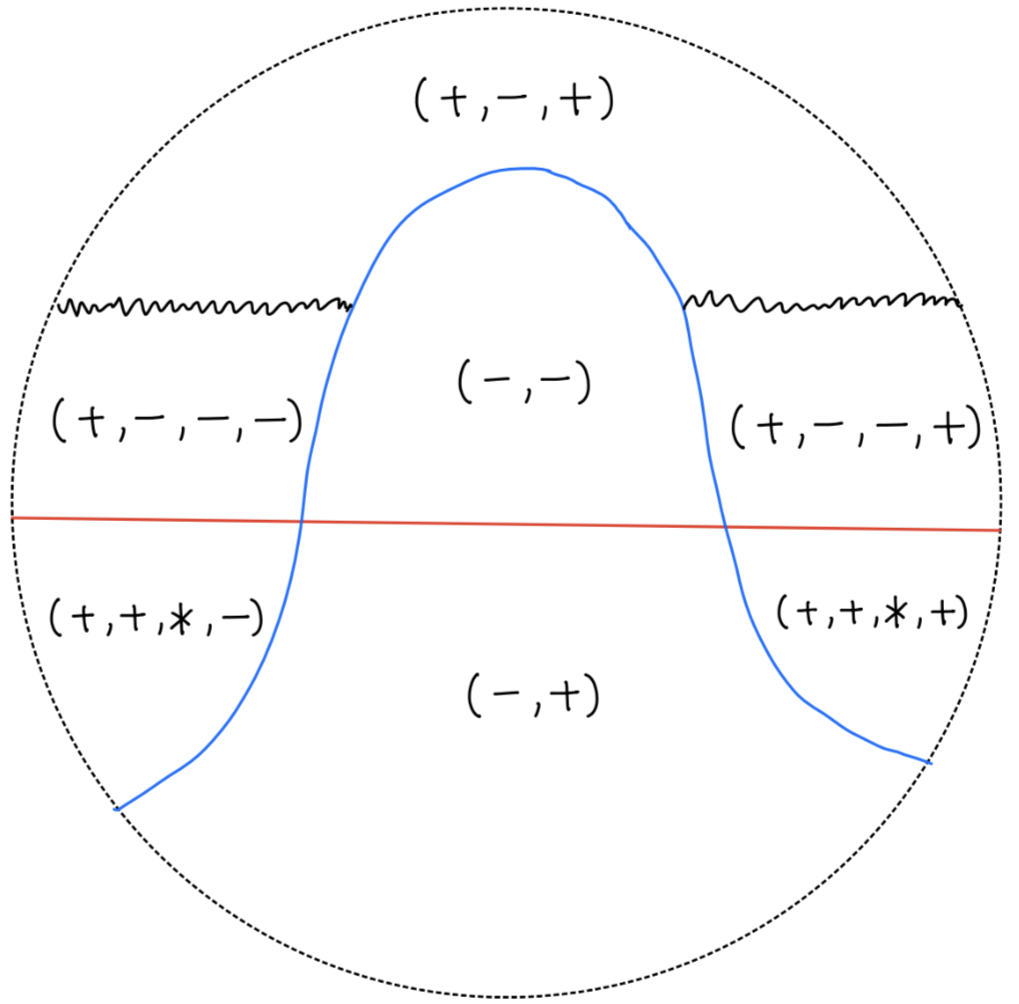
\includegraphics[scale = 0.95]{diagrams/lemma2/1.png} % Adjust the width as needed
    \caption{Your caption here}
    \label{fig:your-label}
\end{figure}

Stalks : \\
- 1 : 0\\
- 2 : $\mathbb{C}\xrightarrow{\times a}\mathbb{C}$\\
- 3 : $\mathbb{C}\xrightarrow{\times b}\mathbb{C}$\\
- 4 : $\mathbb{C}[-1]$ \\
- 5 : $\mathbb{C}$\\
- 6 : $\mathbb{C}$\\
- 7 : 0\\

Generization maps : \\
- 4$\rightarrow$ 1 : zero map \\
- 2$\rightarrow$ 1 : zero map \\
- 3$\rightarrow$ 1 : zero map \\
- 1$\rightarrow$ 5 : zero map \\
- 1$\rightarrow$ 6 : zero map \\
- 7$\rightarrow$ 5 : zero map \\
- 7$\rightarrow$ 6 : zero map \\
- 4$\rightarrow$ 2: 
\begin{tikzcd}
\mathbb{C} \arrow[r, "id"]     & \mathbb{C}  \\
0 \arrow[r]\arrow[u,] & \mathbb{C} \arrow[u,"\times a"]
\end{tikzcd}

- 4$\rightarrow$ 3: 
\begin{tikzcd}
\mathbb{C} \arrow[r, "id"]     & \mathbb{C}  \\
0 \arrow[r]\arrow[u,] & \mathbb{C} \arrow[u,"\times b"]
\end{tikzcd}

- 2$\rightarrow$ 5: 
\begin{tikzcd}
\mathbb{C} \arrow[r,]     & 0  \\
\mathbb{C} \arrow[r, "id"]\arrow[u,"\times a"] & \mathbb{C} \arrow[u,]
\end{tikzcd}

- 3$\rightarrow$ 6: 
\begin{tikzcd}
\mathbb{C} \arrow[r,]     & 0  \\
\mathbb{C} \arrow[r, "id"]\arrow[u,"\times b"] & \mathbb{C} \arrow[u,]
\end{tikzcd}

\begin{figure}[H] % Optional: [h] means here, [t] for top, [b] for bottom, [p] for page of floats
    \centering
    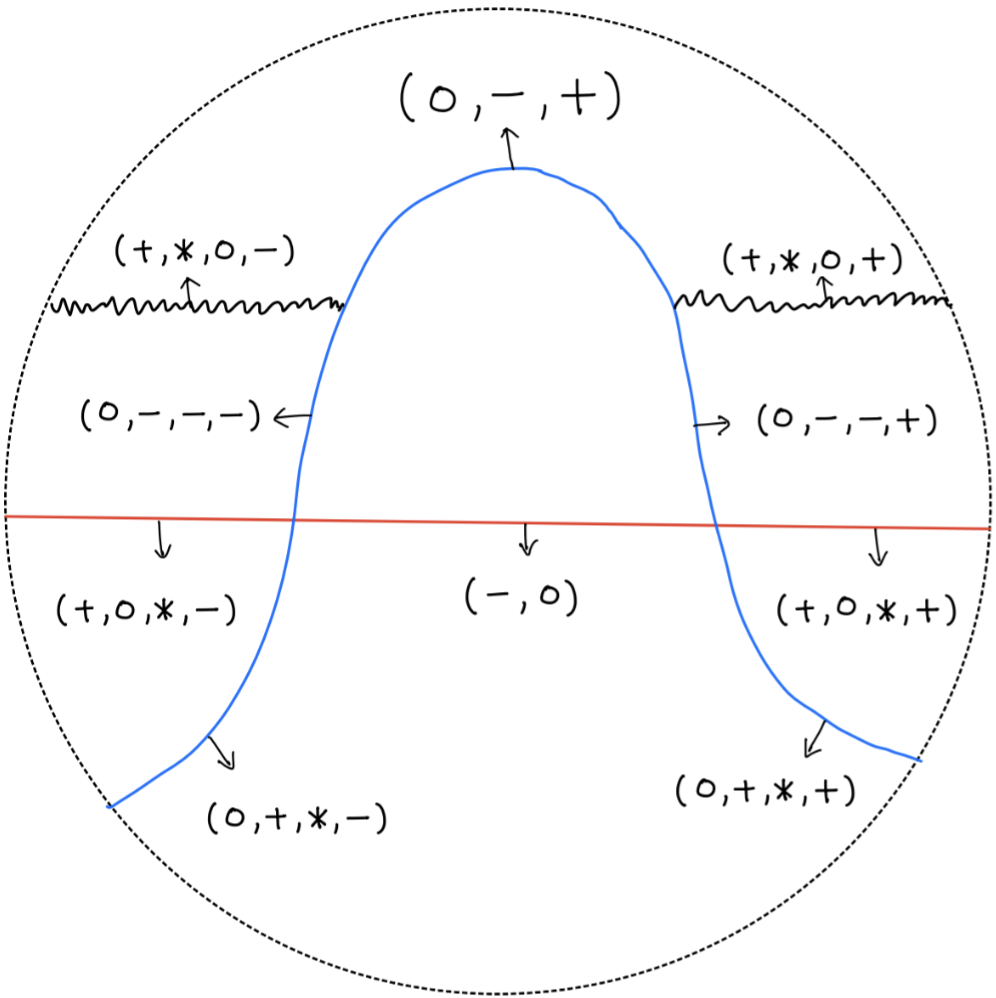
\includegraphics[scale = 0.95]{diagrams/lemma2/2.png} % Adjust the width as needed
    \caption{Your caption here}
    \label{fig:your-label}
\end{figure}

Stalks : \\
1 : 0 \\
2 : $\mathbb{C}\xrightarrow{\times a}\mathbb{C}$\\
3 : $\mathbb{C}\xrightarrow{\times b}\mathbb{C}$\\
4 : $\mathbb{C}$ \\
5 : $\mathbb{C}$ \\
6 : 0

Generization maps : \\

2$\rightarrow$1 : zero map \\
3$\rightarrow$1 : zero map \\
6$\rightarrow$4 : zero map \\
6$\rightarrow$5 : zero map \\
2$\rightarrow$ 4: 
\begin{tikzcd}
\mathbb{C} \arrow[r,]     & 0  \\
\mathbb{C} \arrow[r, "id"]\arrow[u,"\times a"] & \mathbb{C} \arrow[u,]
\end{tikzcd}
\\

3$\rightarrow$ 5: 
\begin{tikzcd}
\mathbb{C} \arrow[r,]     & 0  \\
\mathbb{C} \arrow[r, "id"]\arrow[u,"\times b"] & \mathbb{C} \arrow[u,]
\end{tikzcd}

4$\rightarrow$ 5: $\mathbb{C}\xrightarrow{\times ab^{-1}}\mathbb{C}$\\

We define an isotopy between $\mathfrak{F}$ and $\mathfrak{F}'$ called $isotopy_2$ as follows :

$(\Rn{1})$ The trajectory of the red strand in $D\times [0,1]$ is $\{(x,y,t)\in D\times [0,1]~|~ y = \frac{1}{2}\}$\\
$(\Rn{2})$ The trajectory of blue strand in $D\times [0,1]$ is $\{(x,y,t)\in D\times [0,1]~|~ y = \frac{5}{3}(t-1)x^2 - \frac{5}{4} + \frac{3}{4}\}$. Note that when $t=t_0$, the above set is a parabola passing through $(-\frac{\sqrt{3}}{2}, -\frac{1}{2})$, $(\frac{\sqrt{3}}{2}, -\frac{1}{2})$, $(0, \frac{5}{4}t_0 + \frac{3}{4})$\\

$(\Rn{3})$ The trajectory of the left squiggly line is $\{(x,y,t)\in D\times [0,1]~|~y = \sqrt{\frac{1}{16}-(x+\frac{1}{4})^2}, y \geq \frac{5}{3}(t-1)x^2 - \frac{5}{4}t + \frac{3}{4} \}$\\

$(\Rn{4})$ The trajectory of the right squiggly line $\{(x,y,t)\in D\times [0,1]~|~y = \sqrt{\frac{1}{16}-(x-\frac{1}{4})^2}, y \geq \frac{5}{3}(t-1)x^2 - \frac{5}{4}t + \frac{3}{4} \}$\\

$(\Rn{5})$ The trajectory of the middle squiggly line is$\{(x,y,t)\in D\times [0,1]~|~x=0,y\geq -\frac{1}{2}, y \leq -\frac{5}{4}t + \frac{3}{4} \}$\\

Now I will define sheaf on $D\times [0,1]$ singular supported on $(\Rn{1},\cdots,\Rn{5})$ such that restricted to $D\times\{0\}$($D\times\{1\}$ resp.) is $\mathfrak{F}$($\mathfrak{F}'$ resp.)\\

We can describe the sheaf by assigning stalks to the 7 regions separated by $(\Rn{1},\cdots,\Rn{5})$ and generization maps between them.\\

Let's list the seven regions :

region 1.$\{(x,y,t)\in D\times [0,1]~|~y \geq \sqrt{\frac{1}{16}-(x+\frac{1}{4})^2}, y \geq \sqrt{\frac{1}{16}-(x-\frac{1}{4})^2}, y\geq \frac{1}{2} \}$\\

region2. $\{(x,y,t)\in D\times [0,1]~|~y \geq \frac{5}{3}(t-1)x^2 - \frac{5}{4}t + \frac{3}{4}, y \leq \sqrt{\frac{1}{16}-(x+\frac{1}{4})^2}, y\geq \frac{1}{2} \}$\\

region3. $\{(x,y,t)\in D\times [0,1]~|~y \geq \frac{5}{3}(t-1)x^2 - \frac{5}{4}t + \frac{3}{4}, y \leq \sqrt{\frac{1}{16}-(x-\frac{1}{4})^2}, y\geq \frac{1}{2} \}$\\

region4. $\{(x,y,t)\in D\times [0,1]~|~y \leq \frac{5}{3}(t-1)x^2 - \frac{5}{4}t + \frac{3}{4}, y\geq \frac{1}{2} \}$\\

region5. $\{(x,y,t)\in D\times [0,1]~|~y \geq \frac{5}{3}(t-1)x^2 - \frac{5}{4}t + \frac{3}{4},  y\leq \frac{1}{2}, x\leq 0 \}$\\

region6. $\{(x,y,t)\in D\times [0,1]~|~y \geq \frac{5}{3}(t-1)x^2 - \frac{5}{4}t + \frac{3}{4},  y\leq \frac{1}{2}, x\geq 0 \}$\\

region7. $\{(x,y,t)\in D\times [0,1]~|~y \leq \frac{5}{3}(t-1)x^2 - \frac{5}{4}t + \frac{3}{4},  y\leq \frac{1}{2} \}$\\

Now let's define \\

Stalks:\\

- 1 : 0\\
- 2 : $\mathbb{C}\xrightarrow{\times a}\mathbb{C}$\\
- 3 : $\mathbb{C}\xrightarrow{\times b}\mathbb{C}$\\
- 4 : $\mathbb{C}[-1]$ \\
- 5 : $\mathbb{C}$\\
- 6 : $\mathbb{C}$\\
- 7 : 0\\ 


Generization maps :\\
- 4$\rightarrow$ 1 : zero map \\
- 2$\rightarrow$ 1 : zero map \\
- 3$\rightarrow$ 1 : zero map \\
- 1$\rightarrow$ 5 : zero map \\
- 1$\rightarrow$ 6 : zero map \\
- 7$\rightarrow$ 5 : zero map \\
- 7$\rightarrow$ 6 : zero map \\
- 4$\rightarrow$ 2: 
\begin{tikzcd}
\mathbb{C} \arrow[r, "id"]     & \mathbb{C}  \\
0 \arrow[r]\arrow[u,] & \mathbb{C} \arrow[u,"\times a"]
\end{tikzcd}

- 4$\rightarrow$ 3: 
\begin{tikzcd}
\mathbb{C} \arrow[r, "id"]     & \mathbb{C}  \\
0 \arrow[r]\arrow[u,] & \mathbb{C} \arrow[u,"\times b"]
\end{tikzcd}

- 2$\rightarrow$ 5: 
\begin{tikzcd}
\mathbb{C} \arrow[r,]     & 0  \\
\mathbb{C} \arrow[r, "id"]\arrow[u,"\times a"] & \mathbb{C} \arrow[u,]
\end{tikzcd}

- 3$\rightarrow$ 6: 
\begin{tikzcd}
\mathbb{C} \arrow[r,]     & 0  \\
\mathbb{C} \arrow[r, "id"]\arrow[u,"\times b"] & \mathbb{C} \arrow[u,]
\end{tikzcd}

- 5$\rightarrow$ 6: $\mathbb{C}\xrightarrow{\times ab^{-1}}\mathbb{C}$\\

Below we will prove that this is a well-defined isotopy between $\mathfrak{F}$ and $\mathfrak{F}'$.\\

(proof of well-definedness)